\section{برنامه ریزی مسیر مبتنی بر نمونه برداری}
در بخش های قبلی الگوریتم هایی معرفی شدند که کامل هستند یعنی اگر راه حلی وجود داشته باشد حتما ان را پیدا میکنند اما در عمل این الگوریتم ها وابسته به وضوح نقشه هستند زیرا باید فضای نقشه را که یک فضای پیوسته است برای ان ها به صورت گسسته نمونه گیری کنیم که ممکن است در این عملیات برخی از راه حل ها از بین بروند.

الگوریتم های مبتنی بر نمونه برداری به جای استفاده از روش های ناکامل و یا محاسبه تمام مسیر های ممکن به طور رندوم نقاطی را به یک درخت اضافه می کنند تا زمانی که یک مسیر  پیدا شود و یا محدودیت زمانی به پایان برسد.

\begin{figure}[H]
  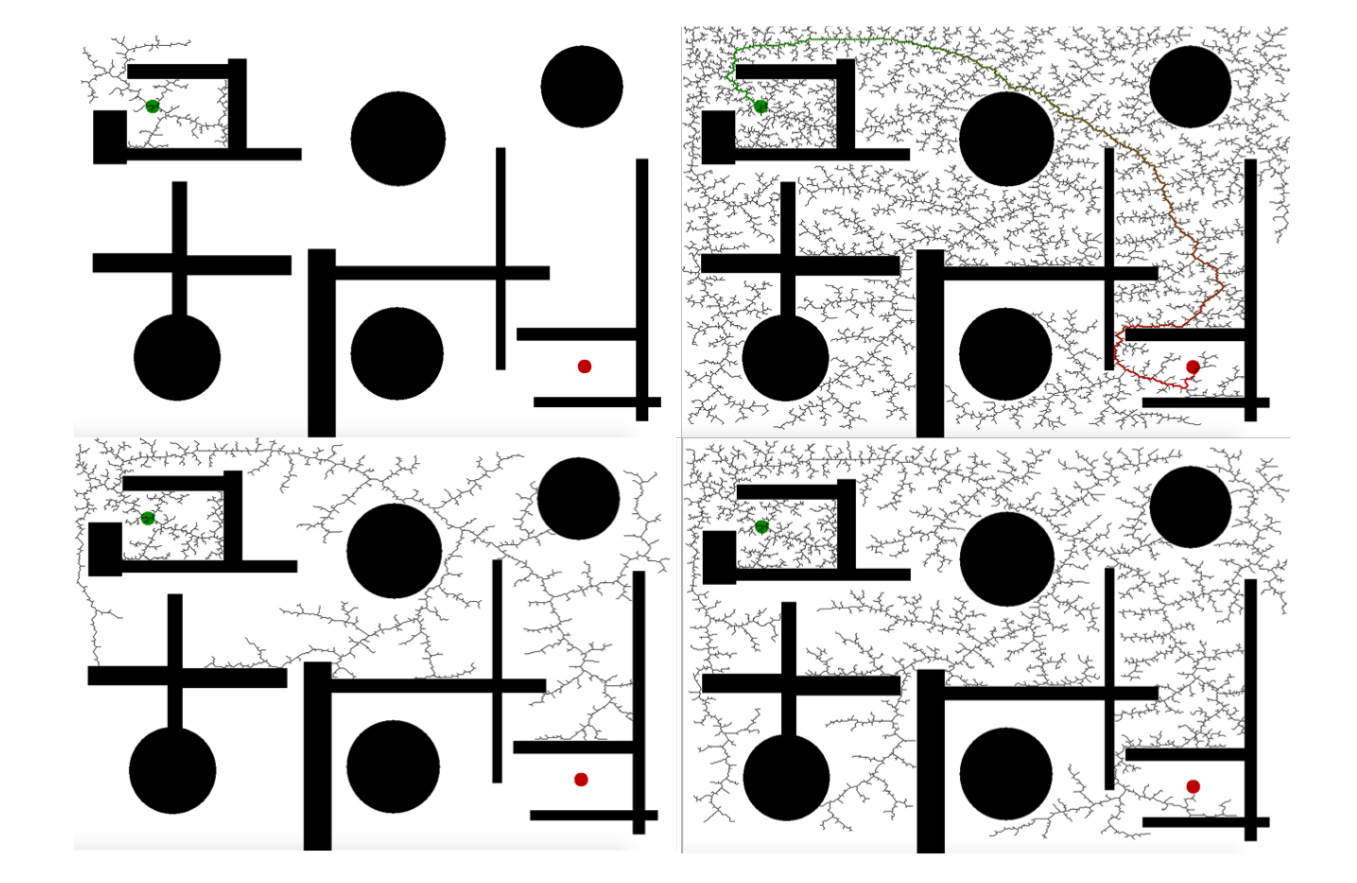
\includegraphics[width = \textwidth]{images/sample.png}
  \caption{
  جستجوی تصادفی روی فضای جستجوی دو بعدی به این شکل که نقاط تصادفی نمونه برداری و به گراف متصل می شوند تا زمانی که یک مسیر ممکن بین شروع و هدف پیدا شود. 
  }
  \label{fig:sample}
\end{figure}
در این الگوریتم ها احتمال پیدا کردن مسیر به سمت یک می رود وقتی که زمان به سمت بی نهایت میل کند.
دو تا از الگوریتم های برجسته در این زمینه عبارتند از:
\begin{itemize}
    \item \lr{Rapidly exploring random trees (RRT)}
    \item \lr{Probabilistic roadmaps (PRM)}
\end{itemize}

الگوریتم اول از نقطه شروع ربات شروع میکند و یک درخت یکتا را به طور تصادفی رشد میدهد تا یکی از شاخه های آن به هدف برخورد کند اما الگوریتم دوم نقاطی را به عنوان نمونه از فضای مورد نظر انتخاب میکند اگر برخورد نداشته باشند ان ها را به هم متصل میکند و سپس با استفاده از الگوریتم های کلاسیک پیدا کردن کوتاه ترین مسیر در گراف کوتاه ترین مسیر بین نقطه شروع و پایان را پیدا میکند مزیت الگوریتم دوم این است که فقط یکبار درخت را می سازد اما در الگوریتم اول هربار درخت باید از اول ساخته شود.

\subsection{الگوریتم پایه}
فرض کنید
$X$
یک وضیعت فضایی چند بعدی باشد. این می تواند بصورت عبارت های انتقالی یا چرخشی یا یک زیرمجموعه یا یک فضای مفصل با یک بعد در هر زاویه ممکن بیان شده باشد. فرض کنید
$G\subset X$
یک توپ چند بعدی در فضای موقعیت به عنوان هدف و $t$ زمان قابل مجاز  در نظر گرفته شود.برنامه ریزی درخت به شکل زیر است: 
\begin{algorithm}[H]
\caption{Tree-planner}
\begin{latin}
\begin{algorithmic}
\STATE $Tree=Init($X$,start)$
\WHILE{$ ElapsedTime() < t$  \textbf{and} $NoGoalFound(G)$}
	\STATE $newpoint = StateToExpandFrom(Tree)$
	\STATE $newsegment = CreatePathToTree(newpoint)$
	\IF {$ChooseToAdd(newsegment)$} 
		\STATE $Tree=Insert(Tree,newsegment)$
	\ENDIF
\ENDWHILE
\RETURN {Tree}

\end{algorithmic}
\end{latin}
\end{algorithm}
این الگوریتم می تواند تا زمانی که زمان مجاز تمام نشده تکرار شود.
همچنین می توانیم فاصله تا مقصد را در هر گره درخت ذخیره کنیم که به کمک آن میتوانیم به راحتی کوتاه ترین مسیر را بیابیم.
چهار نقطه کلیدی در این الگوریتم وجود دارد:
\begin{enumerate}
    \item پیدا کردن نقطه بعدی برای اضافه کردن به درخت
    \item چگونه متصل کردن نقاط جدید به درخت
    \item تست کردن اینکه آیا این مسیر مناسب و بدون برخورد هست یا خیر
    \item پیدا کردن نقطه بعدی برای اضافه کردن
\end{enumerate}
یک روش برجسته این است که یک نقطه تصادفی انتخاب کنیم و آن را به نزدیک ترین نقطه در درخت و یا به هدف متصل کنیم.
این روش نیازمند این است که تمامی نقاط در درخت را سرچ کنیم و نزدیک ترین را به نقطه مورد نظر را بیابیم.
رویکرد های دیگر نقاطی را در اولویت قرار می دهند که درجه خروجی کمتری دارند.
اگر محدودیت هایی روی ربات اعمال شود مثلا ربات به دلیل حمل یک فنجان نتواند مچش را بچرخاند می توانیم این بعد را از فضای جستجو کنار بگذاریم.


\subsection{وصل کردن نقاط به درخت}
به صورت کلاسیک یک نقطه جدید به نزدیکترین نقطه در درخت یا هدف متصل می شود که با محاسبه فاصله این نقاط به راحتی امکان پذیر است اما لزوما کوتاه ترین مسیر را به ما نمی دهد.
اما در الگوریتم RRT روشی وجود دارد که هزینه مسیر را به حداقل میرساند.
در این روش تمامی نقاط درخت که در یک
\lr{ d-ball}
 با شعاع ثابت از نقطه جدید میباشند در نظر گرفته می شوند و بهترین نقطه انتخاب میشود.



\subsubsection{ارزیابی برخورد}
این بخش حدود نود درصد تایم اجرا را در بر میگیرد. یک روش خوب برای بهتر کردن زمان محاسبه روش
\lr{ lazy collision evaluation}
 می باشد. در این روش به جای چک کردن تمام نقاط برای برخورد الگوریتم ابتدا یک مسیر پیدا میکند و سپس بخش های مختلف این مسیر را برای برخورد بررسی میکند و اگر بخش هایی مشکل داشت ان ها را حذف کرده و بخش های بدون مشکل را ذخیره می کند و الگوریتم ادامه می یابد.

